%\section{PRELIMINARY ANALYSIS}

To study the socio-technical congruence of Cargo, I am analysing its package dependency network and the associated technical and social activities of its contributors.
%For this purpose I used Python notebooks and relied on existing data analytics and statistical libraries.
%Focusing on the research questions of Section~\ref{sec:intro}, 
I report some preliminary anecdotal results below. They need to be complemented with proper statistical hypothesis testing, regression and survival analysis, and prediction modeling.
I started to investigate how the presence of commenting activity in a package repository relates to the introduction of dependency to that package.
To do so, I considered all packages in which a new dependency was added,% at some point in time,
and analysed whether commenting activity could be observed in the target package repository \emph{before} or \emph{after} depending on it. Figure~\ref{fig:fig1} summarises the results. One can observe that in more cases commenting activity started after depending on that package. 
An important shift in behaviour can be observed since September 2016, where the number of packages with commenting activity before starting to depend on them is increasing and even exceeds in September 2017 the number of packages with commenting activity after starting to depend on them. Why this occurs remains an open question for now.

\begin{figure}[!bth]
%\vspace{-0.3cm}
    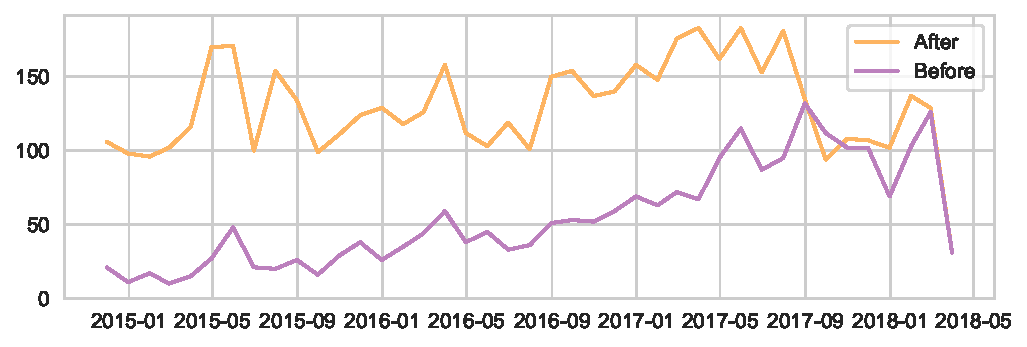
\includegraphics[width=0.9\columnwidth]{Photos/RQ21.pdf} 
\vspace{-0.3cm}
    \caption{Number of package repositories with first commenting activity \emph{before} or \emph{after} starting to depend on a package.}
    \label{fig:fig1}
\end{figure}

\begin{figure}[!tbh]
%\vspace{-0.3cm}
    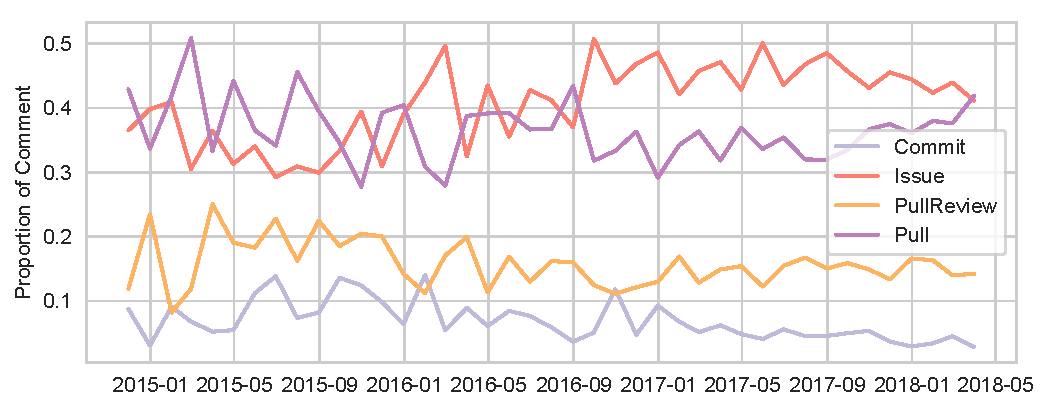
\includegraphics[width=0.9\columnwidth]{Photos/RQ22.pdf} 
\vspace{-0.3cm}
    \caption{Proportion of comment types made in the repositories of packages before starting to depend on that package.}
    \label{fig:fig2}
\end{figure}
\begin{figure}[!tbh]
\vspace{-0.3cm}
    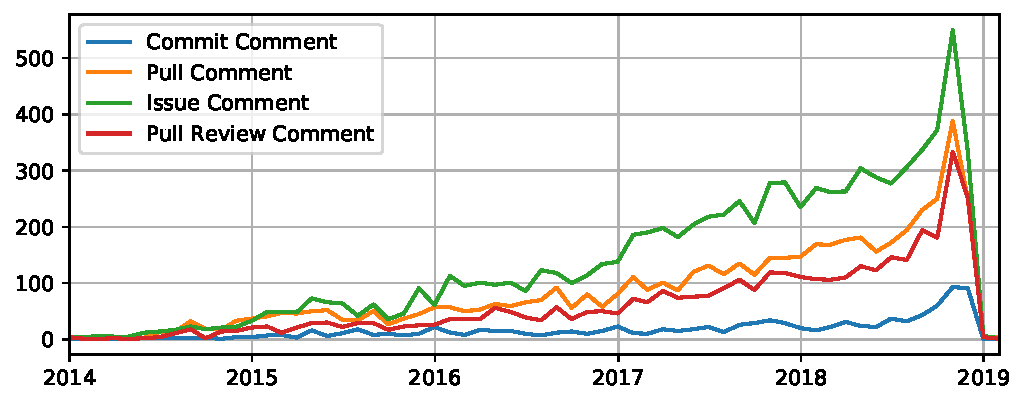
\includegraphics[width=0.9\columnwidth]{Photos/RQ3.pdf} 
\vspace{-0.3cm}
    \caption{Number of cases with comment activity (by comment type) before starting to technically contribute to a package.}
    \label{fig:fig3}
\end{figure}

In order to assess which types of comments (i.e., commit comments, issue comments, pull request comments or pull request review comments) are more likely to lead to the introduction of new package dependencies, I analysed their relative proportion in repositories prior to the addition of a dependency toward those packages. Figure~\ref{fig:fig2} presents these results. 
Among the four types of comments, the proportion of comments on pull requests and issue requests is considerably higher than for commit comments and pull request review comments. I hypothesise that commenting on pull requests and issue requests for a package could serve as a good predictor for adding new dependencies to that package. More detailed statistical analyses are needed to confirm this hypothesis.


I also started to investigate whether social (i.e., commenting) activity on a package repository increases the likelihood to become technically active on that repository (i.e., submitting commits or pull requests). 
Figure~\ref{fig:fig3} presents some preliminary results. Considering the four comment types, issue comments appear to be more likely to result in becoming technically active on a package repository.
The figure shows the number of observations in which the contributor have had a type of comment activity on the package before start to contribute on it.
%{\color{red}TOM: It is impossible to intepret what is shown in Figure 3 due to lack of information. You do not explain what is shown on the y axis, and how the data points  in the figure are computed...}




